\documentclass[a4paper, 12 pt]{article}
\usepackage[utf8]{inputenc}
\usepackage[T1]{fontenc}
\usepackage[slovene]{babel}
\usepackage{lmodern}
%\usepackage{amsmath}
%\usepackage{amsfonts}
%\usepackage{amssymb}
%\usepackage{units}
%\usepackage{eurosym}
%\usepackage{pdfpages}
%\usepackage{comment}
%\usepackage{enumerate}
%\usepackage{mathtools}
\usepackage{mathrsfs}


\usepackage[pdftex]{graphicx}
\usepackage{float}
%\graphicspath{ {/slike/} }

\pagenumbering{arabic}


\begin{document}

\begin{titlepage}

\begin{center}



\Huge
\textbf{Skupina 6: Wiener inverse interval problem}

\vspace{0.5cm}
\large{Projekt v povezavi s predmetom Operacijske raziskave}

\vspace{2.5cm}
\Large
\textbf{Končno poročilo}

\vspace{2.5cm}
\large
Avtorja: \\
\textbf{Tjaša Renko, Darjan Pavšič}

\vfill

\large{Ljubljana, november 2019}


\end{center}
\end{titlepage}


\tableofcontents

\vspace{1cm}

\listoffigures

\pagebreak

\section{Predstavitev problema}

\subsection{Problem P1}

Za fiksno število vozlišč $n$ in drevo $T$ naj bo $\mathscr{T}_{n+1}$ množica vseh dreves na $n+1$ vozliščih, dobljena iz $T$ z dodajanjem lista enemu iz vozlišč $T$. $W(\mathscr{T}_{n+1})$ pa množica vrednosti Wienerjevega indeksa za drevesa iz $\mathscr{T}_{n+1}$. Poiskati želimo tako drevo $T$ na $n$ vozliščih, da bo moč množice $W(\mathscr{T}_{n+1})$ čim manjša (čim večja).


\subsection{Problem P2}

Za fiksno število vozlišč $n$ iščemo drevo $T$ z največjim možnim premerom, da bo veljalo; obstajata list $u$ in vozlišče $w$ iz $T$, da je list $u$, pripet na $v$ in $w$, tak, da z odstranitvijo povezave $uv$ in dodajanjem $uw$ spremenimo vrednost indeksa za 1.

\subsection{Izbira programskega jezika}

Za izvedbo naloge sva se odločila za programski jezik \textit{Python}, za lažje delo z grafi pa sva si pomagala s knjižnico \texttt{networkx}, tako da sva grafe lahko predstavljala kot objekte, sposodila pa sva si tudi vgrajeni funkciji računanja poti med poljubnima vozliščema grafa ter računanja premera. Uporabljala sva tudi knjižnice \texttt{numpy}, \texttt{random} in \texttt{matplotlib}, s katero so grafi tudi vizualno predstavljeni.



\pagebreak

\section{Problem P1}

\subsection{Reševanje}

Zaradi velike časovne zahtevnosti sva kodo ločila na eksaktno, ki je uporabna za majhne $n$ in drugo, kjer si pomagamo s tako imenovanim \textit{simuliranim ohlajanjem}.
\vspace{0.5cm}

V eksaktni kodi najprej dobimo generirane najkrajše poti v drevesu in seznam vsot najkrajših poti ter poračunane Wienerjeve indekse. Nato iz dreves velikosti $n$ generiramo množico dreves z dodanim listom, vrednosti njihovih Wienerjih indeksov pa shranjujemo v seznam. 

\textit{ne vem, kako deluje}

%Na koncu ustvarimo 2 prazna seznama, v enega shranjujemo drevesa, ki so vrnila maksimalno, v drugega pa tista, ki so vrnila %maksimalno vrednosti moči množic Wienerjevega indeksa, kar nas je pri tem problemu zanimalo.

%vsa drevesa z enim vozliščem več (dodan list)
%iščemo drevo z n vozlišči, da bo za n+1 najmanj/največ različnih možnih vrednosti wienerjevega indeksa

\textit{Opis kode s simuliranih ohlajanjem}

\vspace{1cm}

\textit{Časovna zahtevnost - izračunana}

Časovno zahtevnost kode s simuliranim ohlajanjem sva preverila tudi eksperimentalno za nekaj različnih vrednosti $n$.

\begin{figure}[H]
\centering
  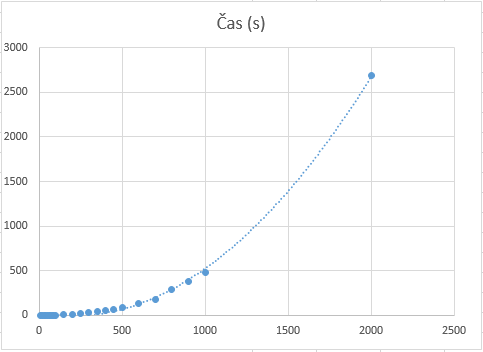
\includegraphics[width=7cm]{p1_casovna_slika.png}
  \caption{Časovna zahtevnost glede na eksperimente pri P1}
  \label{fig:p1_časovna_zaht} 
\end{figure}


\vspace{1cm}




\itshape{ Načrt zdaj je pomikati se po množici ustreznih grafov tako, da najprej narediva par poljubnih dreves na $n$ vozliščih s premerom $n - 2$ in lastnost preveriva za njih, nato vzameva premer $n - 3$ in tako dalje, morda pa tudi na vsakem izmed teh dreves izvesti kakšno metahevristiko ali kaj podobnega. Skrbi naju, da po takšnem postopku dolgo časa sploh ne bi našla grafa z željeno lastnostjo, zato bova morala dobro določiti število izbranih grafov za primerjanje in mogoče zbrati drugačne načine za iskanje.
}

\subsection{Rezultati in povzetek}


\pagebreak

\section{Problem P2}

\subsection{Reševanje}

\normalfont{Za manjše grafe, kjer je možno eksaktno računanje, sva napisala funkcijo za generiranje vseh izomorfnih dreves na $n$ vozliščih ter funkcije, ki najprej iz vseh poberejo tista z iskano lastnostjo, to je spremembo Wienerjevega indeksa za 1 ob odstranitvi ene in dodajanju nove povezave kot v opisu problema, nato pa izmed teh vrne tisto drevo z največjim premerom, če tako sploh obstaja. To je točna rešitev problema, a je časovno zahtevna ne le generacija grafov, temveč tudi računanje premera. Zato sva za večje $n$ tudi tukaj napisala novo kodo.





Primera dveh dreves, ki sva jih dobila z eksaktnim računanjem.}

\begin{figure}[H]
\centering
  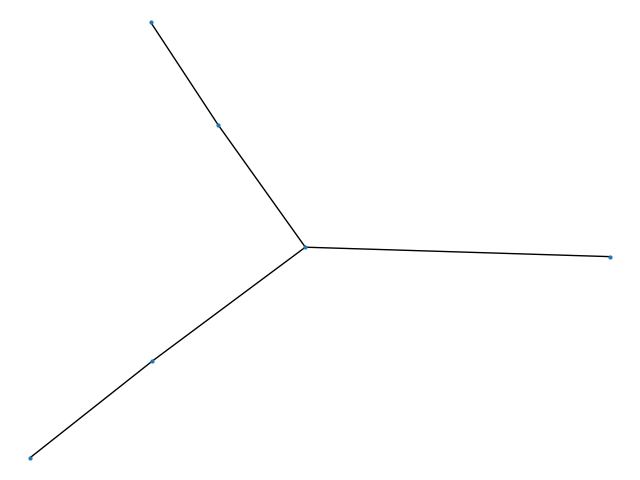
\includegraphics[width=7cm]{drevo6diam4.png}
  \caption{Primer točne rešitve za $n$ = 6, premer = 6}
  \label{fig:graf1} 
\end{figure}

\begin{figure}[H]
\centering
  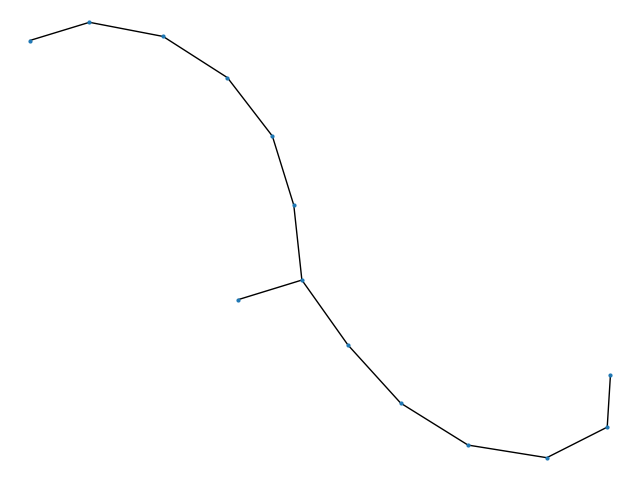
\includegraphics[width=7cm]{drevo14diam12.png}
  \caption{Primer točne rešitve za $n$ = 14, premer = 12}
  \label{fig:graf1}
\end{figure}



\subsection{Rezultati in povzetek}



















\itshape{Za začetek sva potrebovala ustrezne grafe. Ker je izomorfnih dreves na $n$ vozliščih preveč za preverjanje vseh, sva generirala nekaj naključnih s pomočjo Kruskalovega algoritma. Poskusila sva tudi z vgrajenimi funkcijami, a so se izkazale za neuporabne, saj so vračale med seboj preveč podobna drevesa. \newline

Za časovno optimalno računanje Wienerjevih indeksov sva najprej shranila dolžine najkrajših poti med vsakima točkama grafa. Tako sva potem lahko izračunala indeks vsakega posameznega novega drevesa v linearnem času; potrebovala sva namreč le vsoto poti iz vozlišča, ki sva mu dodala list, vsoto vseh poti ter število vozlišč; vse te podatke pa sva že imela. \newline

 Ko sva dobila podatke za na začetku generirana drevesa, sva na vsakem izvedla algoritem za iskanje lokalnih ekstremov v okolici grafa, in sicer vrsto metahevristike z angleškim imenom \textit{simulated annealing}. Ta na vsakem koraku preveri stanje sosednjega grafa in se s padajočo verjetnostjo odloča, ali se bo vanj preselila, hkrati pa shranjuje najboljši rezultat do sedaj. Imela sva težave z definiranjem sosednjega drevesa, zato nameravava preiskusiti par načinov in izbrati ugodnega. Pri prvotnem sva odstranila naključno povezavo, nato pa povezave dodajala in odstranjala, dokler nisva dobila povezanega drevesa, kar se ni izkazalo za učinkovit postopek. \newline

Po končanem algoritmu \textit{simulated annealing} je bilo treba samo še preveriti najboljšega izmed vseh rezultatov, ki jih je podala omenjena metahevristika. Razmišljala sva, da bi na začetku generirala večje število grafov in zadnji algoritem izvedla le na tistih, ki dajejo boljše rezultate, kar bi bilo hitreje. To bo dobro natanko takrat, ko bodo imeli sosednji grafi podobno moč množice $W(\mathscr{T}_{n+1})$, torej želiva to doseči pri novem definiranju sosedov. Poskusila bova z menjavo povezave pri listih, tako kot je to opisano v problemu P2. Nameravava poskusiti tudi na drugačen način, in sicer razmišljava o implementaciji genetskega algoritma. Za to morava razmisliti, kako primerno križati ali kako drugače modificirati ugodni drevesi. Ko bova optimizirala postopke in dobila zadostno število iskanih dreves, se bova morala spomniti še, kako jih primerjati. Za prvih par naravnih števil nameravava tudi preveriti točno rešitev.

\subsection{P2}


\subsection{Zaključek}

Morala bova še implementirati zgoraj omenjene načrte. Sproti bova videla, kaj je potrebno spremeniti, česa se bova znebila in kaj spremenila ali dodala. Poleg iskanja lokalnih optimumov na večjih grafih bova pogledala globalne na manjših ter poskušala sklepati na lastnostih, če se bo pokazal vzorec. Če bo šlo, bova priredila algoritme izdelave prvotnih dreves za testiranje glede na rezultate, ki sva jih dobila na prejšnjih testiranjih.}

\end{document}